\documentclass[letterpaper,11pt]{report}
\usepackage[boxed]{algorithm2e}
\usepackage{algpseudocode}
\usepackage{fullpage}
\usepackage{verbatim}
\usepackage{cite}
\usepackage{setspace}
\usepackage{fancyhdr}
\usepackage{amsmath}


%\usepackage{noReferences}
\usepackage[small]{caption}
\usepackage[leftcaption]{sidecap}
\usepackage{graphics}
\usepackage{color}

\usepackage{hyperref}

%\usepackage{natbib}

\usepackage[dvips]{graphicx}
 % define the title
\graphicspath{ {images/}}

% Paper conservation layout. Long live the trees!!
\setlength{\oddsidemargin}{-0.4mm} % 25 mm left margin
\setlength{\evensidemargin}{\oddsidemargin}
\setlength{\textwidth}{160mm}      % 25 mm right margin
\setlength{\topmargin}{-5.4mm}     % 20 mm top margin
\setlength{\headheight}{5mm}
\setlength{\headsep}{5mm}
\setlength{\footskip}{10mm}
\setlength{\textheight}{237mm}     % 20 mm bottom margin


\setlength{\parskip}{1ex}
\parindent 0in
\def\SAONE{Specific Aim 1}
\def\SATWO{Specific Aim 2}
\def\SATHREE{Specific Aim 3}
\def\SAFOUR{Specific Aim 4}

\def\title{Mytitle}
%\def\titletwo{Thesis Proposal Title Line 2}

\begin{document}





\def\addrone{Your address}
\def\addrtwo{Your city}

\def\degree{M.Tech. in Computer Science with Specialization in Data Engineering}


\def\submissiondate{June 01, 2014}

\def\supervisorone{Haimonti Dutta}

\def\supervisortwo{Srikanta Bedathur}

\def\supervisorthree{Lipika Dey}


%\def\supervisorfour{XXX XXXX }


%\def\supervisorfive{YYY YYYY}

\thispagestyle{empty}

\begin{center}

{\LARGE \bf {FINDING INFLUENTIAL PEOPLE FROM A HISTORICAL NEWS REPOSITORY }

 }  
 \vspace{.3in}
 
 {\Large{Student Name: Aayushee Gupta}} \\  
 \vspace{.1in} 
 IIIT-D-MTech-CS-DE-12-030 \\

% Nov 30, 2011 \\
  
    \vspace{.35in}

  \vspace{.25in}

{Indraprastha Institute of Information Technology\\
New Delhi}

\vspace{.35in}  {\underline{Thesis Committee} \\ \supervisorone         
   \\ \supervisortwo \\ \supervisorthree }\\ \vspace{.35in}


 {Submitted in partial fulfillment of the requirements \\for the Degree of M.Tech. in Computer Science, \\ with specialization in Data Engineering}

\vspace{.2in}

\copyright 2014 SSSSSS SSSSSS \\ All rights reserved \\
\vspace{.8in}


\end{center}


\newpage

\pagestyle{empty}
\vspace*{7.1in} 
Keywords: Gazetteer, Text Mining, Information Retrieval, OCR, Spelling Correction, Historical data, Influential people detection

\newpage

\begin{center}
\section*{Certificate}\label{section:certificate}
\end{center}
%\vspace{3in}
This is to certify that the thesis titled \textbf{``Finding Influential People from Historical new repository"} submitted by \textbf{Aayushee Gupta} for the partial fulfillment of the requirements for the degree of \emph{Master of Technology} in \emph{Computer Science \& Engineering} is a record of the bonafide work carried out by her / him under my / our guidance and supervision in the Data Engineering group at Indraprastha Institute of Information Technology, Delhi. This work has not been submitted anywhere else for the reward of any other degree. \\ \vspace{0.5in}

\textbf{Ms. Haimonti Dutta}\\
\textbf{Indraprastha Institute of Information Technology, New Delhi}
%\doublespacing

\begin{abstract}

 Historical newspaper archives provide a wealth of information. They
are of particular interest to genealogists, historians and scholars
for People Search.

 In this thesis, we design a People Gazetteer from
the noisy OCR text of historical newspapers and identify “influential”
people from it. A People Gazetteer is a dictionary of personal names;
each entry of the gazetteer is  a tuple containing a person name and a
list of articles in which his name occurs.

To build the People Gazetteer, we first spell correct the noisy text
using an edit distance based algorithm. A novel N-gram based
evaluation algorithm is designed for measuring the performance of the
spell corrector. Next, a Named Entity Recognizer is run on the text of
each article to identify person entities and an LDA-based topic
detector to assign categories to articles. To identify influential
people from People Gazetteer across each category, we define the notion
of an Influential Person Index (IPI) and rank based on it. Our corpus
is a sample of 14020 newspaper articles (roughly two months’ data)
obtained from “The Sun” newspaper in the Chronicling America project.

\end{abstract}

\newpage
\pagestyle{empty}


\newpage



\section*{Acknowledgments}\label{section:acknowledgments}
\pagestyle{plain}
\pagenumbering{roman}

XXXXXX XXXXXX XXXXXX XXXXXX XXXXXX XXXXXX XXXXXX XXXXXX XXXXXX XXXXXX XXXXXX XXXXXX XXXXXX XXXXXX XXXXXX XXXXXX XXXXXX XXXXXX XXXXXX XXXXXX XXXXXX XXXXXX XXXXXX XXXXXX XXXXXX XXXXXX XXXXXX XXXXXX XXXXXX XXXXXX XXXXXX XXXXXX 

\newpage

\tableofcontents
\listoffigures 
\listoftables

\newpage

\newpage

\newpage
\mbox{}


%\doublespacing

\chapter{Introduction}\label{chapter:introduction}
%\pagestyle{fancy}
\pagenumbering{arabic}
\setcounter{page}{1}
\onehalfspacing



\section {Motivation}

Newspapers are rich sources of history and millions of pages of historical newspapers have been digitized \cite{Allen_10} in recent years. A national program to develop an Internet-based, searchable database of U.S. newspapers called the National Digital Newspaper Program (NDNP) was setup in 2004 as a partnership between the National Endowment of Humanities (NEH) and the Library of Congress. Since then, several public and for-profit sectors have also digitized newspapers at a rapid pace making text from historical records available at a staggering rate. To deal with this wealth of information, scholars have mainly focused on text mining and information retrieval techniques followed by visualization of patterns extracted from the records \cite{McKeown_1995, Radev99c, mckeown2002tracking, dutta2011learning, Berberich_2007, khurdiya2011multi, shahaf2010connecting}. 


\begin{figure*}[t]
\begin{center}
%\mbox{
\subfigure[GenealogyBank]
{
%%\includegraphics[width=0.6\columnwidth]{odds_20070813_160000rb_M.pdf}

\includegraphics[width=0.43\textwidth, height=0.23\textheight]{genealogy.jpg}
\label{fig:gen}
}
\subfigure[FamilySearch]
{
%%\includegraphics[width=0.8\columnwidth]{20070813-C1-7d-roc.pdf}
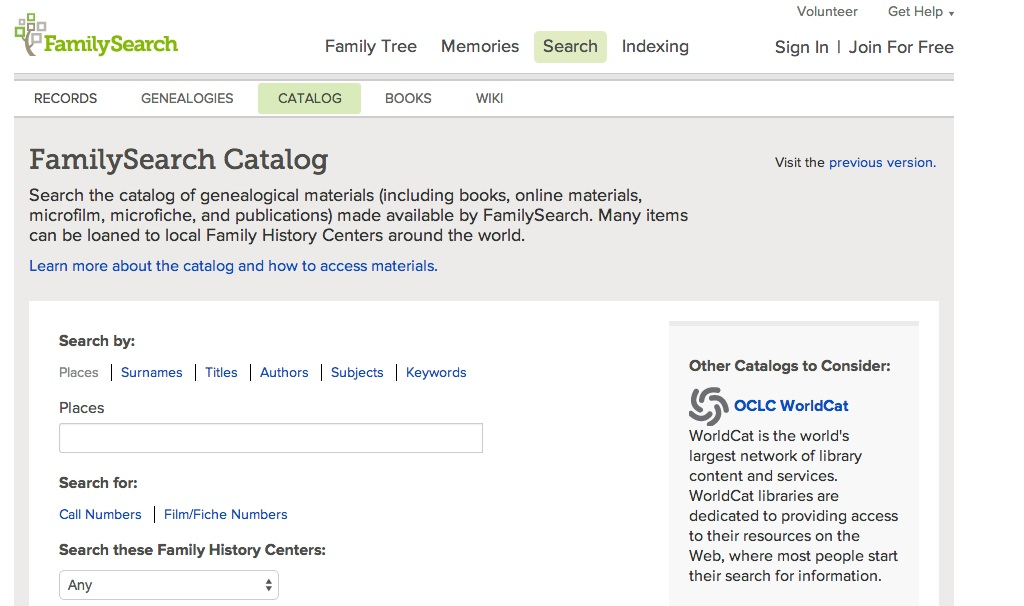
\includegraphics[width=0.43\textwidth, height=0.23\textheight]{FamilySearch}
\label{fig:fam}
}
%}
\caption{Two examples of online People Search Tools which utilize historic newspaper archives, military records, petitions, obituaries, census records and other forms of petitions to match proper nouns.}
\label{figSearch}
\end{center}
\end{figure*}

An important use of historical newspapers is for People Search\cite{BilenkoMCRF03,Friedman_92}) -- for example, to find important people and track the timelines of news articles related to them. Several websites like Genealogy Bank\footnote{http://www.genealogybank.com/gbnk/}, FamilySearch\footnote{https://familysearch.org/}, Newspaper Archives\footnote{http://newspaperarchive.com/}, Ancestry\footnote{http://www.ancestry.com/} provide people search service that include obituaries, birth and death lists, newspaper articles, military records, Revolutionary and Civil War pension requests, census records, land grants and other forms of petitions. Figure~\ref{figSearch} shows two such tools available online.

%Existing literature also deals with the problem of spelling variations in people names -- solutions include use of Soundex\footnote{http://www.myheritage.com/FP/Company/megadex.php} technology that given a query, returns everything that ``sounds like" what the query term. Face recognition algorithms, video and audio clips have been used to enhance search. However research in this domain is still in its nascent stages.


%Information related to a person can be extracted from online freely available historical archives of newspapers for which the text requires cleaning and preprocessing to make the information available in the required format.
  
To the best of our knowledge, the problem of finding \emph{influential} people from historic newspaper archives has not been studied before. This exercise, however, opens up a wide range of possibilities -- for example, news articles related to the influential person can also be linked to a Wikipedia page entry to find out relevant details or build influential people networks that can learn about entities involved in historical events. 

\section{Problem Description}
\label{problem}
%%DOUBT: DIFFERENCE BETWEEN AIM AND PROBLEM DESCRIPTION? DO THEY NEED TO BE MENTIONED SEPARATELY?


The goal of this research is to find and rank influential people across multiple topic categories in historical newspaper OCR archives.


%DOUBT:  IS IT OK TO MENTION THESE DETAILS HERE OR THEY SHOULD BE WRITTEN IN RELATED WORK?
%The problem of finding influential people in this scenario is a novel one as much of the research work deals with identification of influential nodes in social networks or marketing and diffusion research. This research does not involve finding influential people in terms of their influence on their peers\cite{watts2007influentials} or influence propagation in a social network \cite{kempe2003maximizing} which is how the concept of influence is used in general.   

 An influential person can be defined as ``a person whose actions and opinions strongly influence a course of events". This allows us to link an influential person with a list of articles that s/he occurs in.
 A person may also be considered influential if s/he gets talked about frequently in news articles. The problem can be also be phrased as identifying and ranking \emph{popular} people across various categories in the news domain. 
 ``Popularity" has been defined in other domains by counting number of votes, tweets, citations and followers. \cite{cheng2014can} but similar measures are not applicable in a newspaper setting where only the newspaper articles mentioning multiple people names are available.  
 
We divide the the problem of finding influential people into the following subproblems:
\begin{itemize}
\item \textbf{Problem 1: } Spell Correction and Cleaning of OCR text
\item \textbf{Problem 2: } Development of a People Gazetteer -- develop an organized structure in order to ease the process of identification of influential people.
\item \textbf{Problem 3: } Influential People Identification -- define the criteria for identifying and ranking people as ``influential".
\end{itemize}
  
%Each of the above problems require consideration of the dataset size and characteristics along with the newspaper environment in mind. 
\begin{figure}[h]
\centering
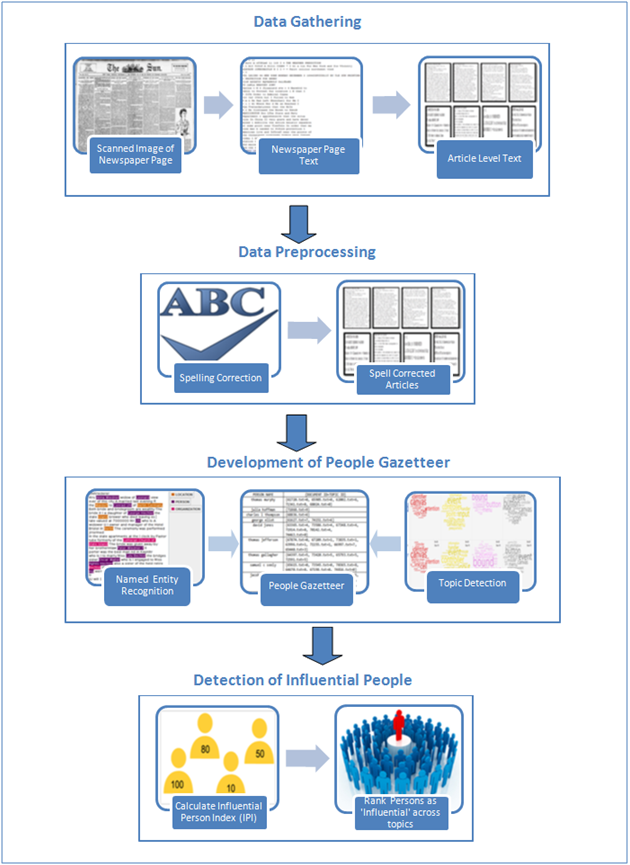
\includegraphics[width=0.6\textwidth, height=0.5\textheight]{framework3}
\caption{Research Framework showing components of proposed solution}
\label{fig:framework}
\end{figure} 

\section {Research Framework}

We propose the following solution framework in Figure~\ref{fig:framework} for finding influential people from a historical news repository. Each component is briefly described as follows:

\begin{enumerate}
\item \textbf {Data Gathering}:  
This component describes the source of data along with relevant statistics. It also includes descriptions of how the page level newspaper images are converted to text through OCR followed by article level segmentation. The different types of OCR errors encountered in the data are also described. This component is further discussed in Chapter ~\ref{chapter:data description}.

\item \textbf {Data Preprocessing}:
This component describes the preprocessing applied on the news articles. It describes relevant spelling correction algorithms, and then presents a novel algorithm for evaluation of the results. This component is further discussed in detail in Chapter ~\ref{chapter:data preprocessing}.

\item \textbf {Development of People Gazetteer}:
This component describes the process of development of people gazetteer which involves Named Entity Recognition in order to find person entities. This is followed by topic detection using LDA to assign topics to news articles and link both to obtain an organized structure. This component is discussed in detail in Chapter ~\ref{chapter:people gazetteer}.

\item \textbf {Influential Person Identification}:
This component defines an ``Influential Person Index" (IPI) that incorporates several criteria for identifying and ranking of ``influential people" across newspaper topics. Details about IPI, ranking and final results with some case studies are discussed in Chapter ~\ref{chapter:influential people detection}.

\end{enumerate}
 


%DOUBT: EITHER WRITE AS WE AIM TO ANSWER THESE QUESTIONS IN THIS RESEARCH OR WE DIVIDE THE PROBLEM INTO THESE SUBPROBLEMS...
%We aim to answer the following questions related to the problem of finding influential people with this research:
%Question 1 : How to deal with OCR data consisting of extremely noisy text for such a task?
%Question 2 : How to develop and use an organized structure for easy identification of influential people?
%Question 3 : Who are `influential persons" in a newspaper scenario and how to rank them?


%DOUBT: NOT SURE WHETHER RESEARCH FRAMEWORK SHOULD COME FIRST OR NOVEL CONTRIBUTION?
\section{Research Contributions}
\label{intro:rc}
This thesis has the following novel contributions:
\begin{enumerate}
\item A new algorithm for \emph{evaluation} of the performance of the spelling correction algorithm is presented. 
\item Development of the People Gazetteer -- an organized dictionary of people names and a list of articles in which the name occurs along with the corresponding topic of each article to facilitate identification of influential people.
\item Define an Influential Person Index (IPI) and metrics for its calculation in order to identify and rank influential people. Case studies of the top-K influential people detected are also discussed and verified with Wikipedia data. 

\end{enumerate}


 

\chapter{Related Work}


Different types of gazetteers are discussed in \footnote{http://gate.ac.uk/sale/tao/splitch13.html}. They define gazetteers as set of lists containing names of entities such as cities, organisations, days of the week, etc. along with their types. They use gazetteer either as set of entity list or as a processing resource used to find occurrences of the entity names in text, e.g. for the task of named entity recognition. We use this definition to develop our People Gazetteer as a processing resource that finds person name entities from the news articles repository, associates each unique person entity from news articles with a list of articles of its occurence and their respective topic.

Gazetteer lists are also discussed in \cite{carlson2009learning} where they are used for learning name entity tagger using partial perceptron and aid in performing better NER compared to CRF based entity taggers.
\cite{zhang2009novel} discuss automatic generation of gazeteer list by finding entities with similar type labels from Wikipedia articles which can further be used for the purpose of NER. The evaluation is done over scientific domain of Archaeology considering subject, temporal terms and location as named entities but no evaluation is presented for person entities.
There is also no relevant work that builds or uses historical person names gazetteer list for data mining that we know of.

\cite{lloyd2005lydia} discuss their approach for designing a news analysis system \footnote{http://www.textmap.com} where information about several types of entities can be searched. They allow searching over all entities found in the news sources, present juxtaposition for each entity, i.e., other entities mentioned in context, temporal and spatial analysis, popularity time series graph in terms of number of number of references and coreference names for the entity.
But they do not focus on finding influential entities in which respect our research is different from their work.

We discuss more related work regarding data preprocessing using Spelling correction algorithms in Section ~\ref{spell:rw} and finding influential people in Section ~\ref{influential:rw}.






\chapter{Data Description}
\label{chapter:data description}

This chapter describes the dataset used for developing the People Gazetteer. Following sections provide details of data source, characteristics and some data statistics.

\section{Data Source} 

The dataset has been taken from Chronicling America.
\noindent \emph{Chronicling
America}\footnote{\texttt{http://chroniclingamerica.loc.gov/}} is an
initiative of the National Endowment for Humanities (NEH) and the
Library of Congress (LC) whose goal is to develop an online,
searchable database of historically significant newspapers between
1836 and 1922. The New York Public Library (NYPL) is part of this
initiative and has scanned 200,000 newspaper pages published between
1890 and 1920 from microfilm.

In order to make a newspaper available for searching on the Internet,
the following processes used in \cite{dutta2011learning} must take place: (1) the microfilm copy or
paper original is scanned; (2) master and Web image files are
generated; (3) metadata is assigned for each page to improve the
search capability of the newspaper; (4) OCR software is run over high
resolution images to create searchable full text and (5) OCR text,
images, and metadata are imported into a digital library software
program. The scanned newspaper holdings of the NYPL offers a wealth of
data and opinion for researchers and historians.

The newspaper titles and digitized pages available through the
Chronicling America website can be searched using the OpenSearch
protocol\footnote{\texttt{http://www.opensearch.org/Home}}.
Unfortunately, the current search facilities are rudimentary and
irrelevant documents are often more highly ranked than relevant ones.
The newspapers are scanned on a page-by-page basis and article level
segmentation is poor or non-existent; the OCR scanning process is far
from perfect and the documents generated from it contains a large
amount of garbled text. In a bid to serve its patrons better, the New
York Public Library employed human annotators to clean headlines of
articles and text, but the process of manually reading all the old
newspapers article-by-article and cleaning them soon became very
expensive. 

\section{Data Characteristics}
An individual OCR text article has at least one or more of the following types of spelling errors:

\begin{figure}[hbt]
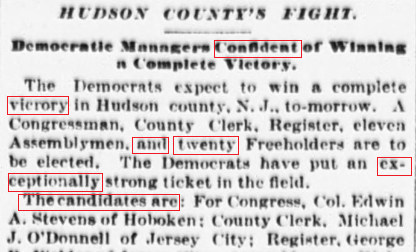
\includegraphics[scale=0.75]{originalimage}
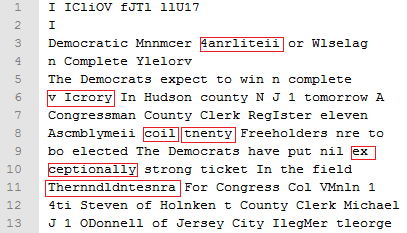
\includegraphics[scale=0.80]{ocr}
\caption{Scanned Image of a Newspaper article (left) and its OCR raw text (right)}
\end{figure}

\begin{description}
 \item[$\bullet$Real word errors] include words that are spelled correctly in the OCR text but still incorrect when compared to the original newspaper article image. For example: In Figure 3.1, the word ``coil"  has been correctly spelled in the OCR text  but should have been ``and" according to the original newspaper article. 
 \item[$\bullet$Non-real word errors] include words that have been misspelled due to some insertion, deletion, substitution or transposition of characters from a word. For eg. In Figure 3.1, the word ``tnenty" in the OCR text has a substitution error (`n' should have been `w') which is actually ``twenty" according to the original newspaper article.
 \item[$\bullet$Non-word errors] include words that have been spelled incorrectly and are a combination of alphabets and numerical characters. For example: In Figure 3.1, the word ``4anrliteii" which is a combination of alphabets and number and should have been ``confident" as per the original newspaper article.
\item[$\bullet$New Line errors] include words that are separated by hyphens where part of a word is written on one text line and remaining part in the next line. For example: In Figure 3.1, the word ``ex-ceptionally" where ``ex" occurs on one line while ``ceptionally" in the next and due to no punctuation in the text, they are treated as separate words in OCR text.
\item[$\bullet$Word Split and Join errors] include words that either get split into one of more parts or some words in a sentence get joined to a make a single word. For example: In Figure 3.1, the word ``Thernndldntesnra" in the OCR text is actually a combination of three words ``The candidates are" while the words ``v Icrory" are actually equivalent to a single word ``victory" when compared with the original news article.
\end{description} 

\section{Data Statistics}
The OCR text available from Chronicling America website is on a page by page level and no article level segmentation is provided. OCR text dataset is therefore, taken from a PostgreSQL database where article level segmentation of page-level OCR text from Chrocling America is available for two months of articles of ``The Sun" newspaper from November-December 1894 consisting of 14020 news articles with a total of 8,403,844 tokens. The newspaper database ER diagram \footnote{https://power.ldeo.columbia.edu/twiki/pub/Incubator/BodhiDBDesign/Final ERD.pdf }
is used to extract the required articles text from the database by dumping complete dataset and extracting individual articles linetext based on their unique ID. The individual text articles generated from the database do not have any punctuation and contain a large amount of garbled text containing above mentioned OCR errors.


\chapter{Data Preprocessing}
\label{chapter:data preprocessing} 

 
This chapter describes the preprocessing steps applied on the historical news articles.
The garbled OCR text makes data preprocessing mandatory before application of any text mining algorithms. 

\section{Spelling Correction}

Several kinds of spelling errors exist in the data as described in chapter~\ref{chapter:data description}. This chapter first provides a brief review of spelling correction algorithms that exist in literature (Section~\ref{spell:rw}); Section~\ref{spell:algo} describes the algorithm used in this research and evaluation results on the OCR dataset are presented in Section~\ref{spell:eval}.

% DOUBT: Do the following lines need to be removed?
%The garbled OCR dataset  needs to be refined by correcting the text with the help of a human editor manually or automatic spelling corrector. Due to the huge size of dataset, human editing would be extremely time consuming and expensive making it impossible and indicating requirement of a spelling correction technique. 
%The spelling correction of person named entities in the dataset also requires special consideration so that the person named entities with correct spellings get detected as a result which is the main aim of this research.


\subsection{Related Work}
\label{spell:rw}

Kukich\cite{kukich1992techniques} comprehensively discusses various spelling correction techniques based on Non word, Isolated word and Real word spelling errors. N-gram analysis, Dictionary lookup and Probabilistic techniques are used for correcting isolated and nonword errors while Context-Dependent techniques are used mostly for correcting real word errors including the correction of word split and join errors \cite{elmi1998spelling}.

 N-gram techniques work by examining each n-gram in the text string and comparing against a pre-compiled table of n-gram statistics to retrieve the correct word while Dictionary look up techniques directly check whether the text string appears in the dictionary using string matching algorithms. Both techniques require a dictionary or a large text corpus and take frequency of n-grams or word occurrence into account in order to find the correct spelling \cite{strohmaier2003lexical}, \cite{ringlstetter2007text}.
 Probabilistic techniques use transition and word confusion probabilities to estimate likelihood of the correction in order to rank and retrieve correct word spelling.

On the other hand, Context-dependent techniques require contextual information and use either extensive NLP techniques or Statistical Language Modeling (SLM) for spelling correction.
Bassil and Alwani\cite{bassil2012ocr} use Google 1-5 gram word dataset to gain context information in order to determine the correct words sequence in the text for correction.
Tong and Evans\cite{tong1996statistical} use SLM approach involving information from letter n-grams,character confusion and word bi-gram probabilities to perform context sensitive spelling correction obtaining a 60 percent error reduction rate. 

All these spelling correction techniques have developed over time and have been used in combination to achieve improved accuracy \cite{brill2000improved}. \cite{agarwal2013utilizing} use a combination of Google suggestions, LCS and character confusion probabilities for choosing the correct spelling on a small set of historical newspaper data and achieve recall and precision of $51\%$ and $100\%$ respectively.


Edit distance approach, suggested initially by Wagner and Fischer\cite{wagner1974string}, is a dictionary lookup approach commonly used for OCR data correction because of the large number of substitution errors in OCR data  \cite{kukich1992techniques}\cite{christen2006comparison} which can be corrected using this technique. String edit distance approaches with faster correction are discussed in \cite{marzal1993computation},\cite{schulz2002fast}  with variants like Levenshtein automata and normalized edit distance.

Personal name spelling correction has also been studied separately including comparison among various techniques indicating that there is no one single technique that outperforms all others though pattern matching techniques result in better matching quality compared to phonetic encoding techniques\cite{christen2006comparison}. Almost all the personal name spelling correction techniques use personal names directory/dictionary for matching against wrongly spelled names in the dataset or queries in case of People Search \cite{udupa2010hashing}. 
  
%CHANGES MADE HERE. ADDED A LINE REGARDING PERSONAL NAMES CORRECTION AND MOVED RELATED WORK REGARDING EVALUATION ALGORITHM TO SECTION 4.1.3.
 We use edit distance algorithm for spelling correction because of its speed and ability to correct OCR errors compared to the n-gram approach \cite{chattopadhyaya2013fast}. Context-dependent spelling correction is not used because of unavailability of n-gram words corpus or ground truth dataset containing OCR and true word pairs. Our edit distance algorithm also uses an enhanced dictionary for look up to give significance to personal names spelling correction in the dataset. 


\subsection{Spelling Correction Algorithm}
\label{spell:algo}

The Edit Distance algorithm based on Levenshtein distance\cite{levenshtein1966binary} has been used for spelling correction. It is an isolated word correction technique that uses dictionary based-look up method and distance between strings for matching the text and correcting it. An ``edit distance" corresponds to the minimum number of insertions, deletions, and substitutions required to transform one string into another. The algorithm corrects Non-Real Word spelling errors up to an edit distance of 2 , i.e. , it corrects words which have spelling errors that can be corrected by making at most 2 operations of insertion, deletion and substitution of letters in the word. The choice of 2 is governed by the trade off between algorithm runtime and quality of spelling correction. A bigger value improves the spelling correction accuracy but increases the runtime also while a smaller value decreases accuracy and the algorithm runtime.
The spelling corrector has been designed as suggested by Peter Norvig \footnote{ http://norvig.com/spell-correct.html}. The algorithm requires a dictionary which is used to check if each word of the text exists in it or not. If the word already exists in the dictionary then no change is made to the word and if not, then a candidate list of words is created from the word to be corrected by inserting, substituting or deleting up to 2 letters from it.  This list of words is again checked for in the dictionary and returned as suggestions for the word to be corrected. The correction is made with the word formed from lowest edit distance and occurring with more frequency in the dictionary. This makes the edit distance algorithm dependent on the type of dictionary chosen for correction which means the dictionary must be well chosen for spelling correction of a specific document collection. The algorithm runs faster by reading the dictionary only once and keeping a data structure in memory for its word counts which can be referred to whenever a word comes up for correction.

\subsection{Spelling Correction Algorithm Evaluation}


There has not been much related work regarding automatic evaluation of word-by-word post spelling correction on OCR dataset consisting of Word Split and Join errors. Semi-automatic spelling correction system is discussed in \cite{taghva2001ocrspell} that corrects these errors but requires user interaction in order to perform complete correction and system evaluation. Rice\cite{rice1996measuring} discusses OCR errors similar to the ones in our dataset. Their algorithm evaluates edit distance spelling correction by estimating word accuracy defined as the percentage of correctly recognized words; the length of LCS between correct and incorrect strings on a page by page level is used as the relevant metric. The evaluation strategy works correctly but the definition of accuracy does not give a complete coverage of the spell correction as it does not provide any information on the errors missed by the spelling corrector.

For evaluation on our dataset, the raw OCR text and OCR text after application of spelling correction algorithm needs to be compared with the original newspaper text. The OCR text is extremely garbled with Word Split and Join errors due to which word-to-word alignment with the original newspaper text is impossible. For this purpose, a novel algorithm called SCE (Spelling Correction Evaluation) based on N-gram approach is proposed for automatic evaluation of the corrected text word-by-word against the manually corrected subset of the news articles dataset. 

Following sections describe the evaluation parameters for estimating the performance of Spelling Corrector on the OCR dataset used along with the SCE algorithm:

\subsubsection{Evaluation Parameters}

\begin{description}

 \item[$\bullet$Accuracy]
 The evaluation metric used for measuring the performance of Spelling correction algorithm is Accuracy which requires calculation of number of OCR errors that got corrected when compared to the original scanned newspaper text. The measure has been chosen so as to include the complete text coverage and not just check for words that got corrected after spell correction as in the latter case, the  number of FP and TN get missed which won't give the correct measure of how well the spell corrector works. The formula used for calculating Accuracy is defined by Manning and Schutze,1999 (p.268-269) as follows:

$Accuracy=  \dfrac{TP+FP} {TP+ FP + TN + FN}$


where 

TP=Number of True Positives,

TN=Number of True Negatives,

 FP=Number of False Positives,

 FN=Number of False Negatives. 

The aim of the SCE algorithm is to make a word-to-word correspondence between the OCR corrected text and the original OCR text and to mark each token in the OCR text as a TP, FP, TN or FN. Reynaert and Martin\cite{reynaert2008all} suggest a way to define these terms by distinguishing between correct words and incorrect words in the text through the set of non-target, target and selected words and use Precision and Recall evaluation measures for measuring performance of spelling correction. 

According to our spelling corrector, a ``true positive" is said to occur when a word from the OCR text gets corrected and the corrected spelling matches the one in original article text while a ``false positive" occurs if the corrected spelling does not match the corresponding word in the original article text. A ``true negative" occurs when a word does not get corrected by the algorithm as it is already correct and matches the correct word in the original text also. On the other hand, a ``false negative" occurs when the algorithm is unable to correct the word (there is no change in spelling of the word) and it does not match the corresponding word in the original text but should have been corrected.



\item[$\bullet$Time taken for Spelling Correction]
Time is also an essential parameter while measuring the performance of spelling correction. Since the dataset is quite large, it is important that the algorithm does not take too long to correct an article and needs to be parallelized in case it takes more time for correction.


\item[$\bullet$Person Names Detection Rate]

The spelling correction algorithm is evaluated on the basis of another parameter which is used to consider the special case of person entity names spelling correction, as the main goal of research is to detect these names with correct spellings.
Person Names Detection Rate can be defined as the ratio of person names recognized through Named Entity Recognition before spelling correction process and the total number of person names recognized in the original newspaper articles.

$Person Names Detection Rate=\dfrac{ \text{Person Names recognized before/after spelling correction}} {\text{ Person Names recognized in original newspaper articles}} $

\end{description}

\subsubsection{SCE (Spelling Correction Evaluation) Algorithm}

The SCE algorithm is based on an N-word grams approach. To make the correspondence between corrected and original OCR text, a window of n-word grams in the scanned image text article is considered (Original.txt) which can be seen in a digrammatic representation in Figure 4.1.

\begin{figure} [!htb]
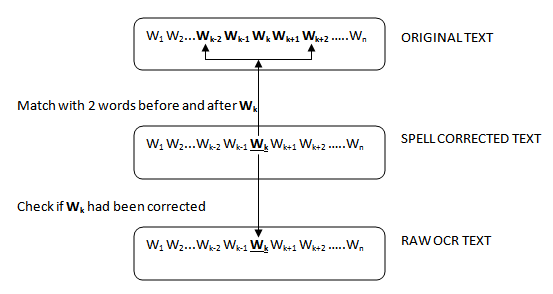
\includegraphics[scale=0.8]{ngram}
\caption{Schematic diagram for alignment of spell corrected article text with original article text for a word $W_{k}$}
\end{figure}
For each token in the spell corrected text (Corrected.txt), the corresponding token  in the scanned text article along with 2 tokens before and 2 tokens after it are considered for alignment\footnote{ The choice of 2 is based on the Word Split and Join errors in the dataset. Choosing n=2 allows a window of words to be considered to make up for the alignment lost because of Word Split and Join errors.}.
If the token being considered matches with any of these words in the scanned text article words window and its spelling has been corrected when compared to the corresponding token in raw OCR text (OCR.txt), then it is marked as a ``True Positive" which is actually rewarding the Spell corrector for making the correct spelling change. A ``False Positive" is marked if it does not match any of the words despite its spelling being corrected. If the token being considered matches any of the words in the words window but no spelling correction has been made for it, then it is marked as a ``True Negative" and if it does not match any word in the window and the spelling corrector also did not correct it, then it is marked as a ``False Negative" as the word got missed by the corrector. 

Several cases could occur like difference in the lengths of linetext between OCR and Original text or while considering the first, second or the last tokens from the Corrected text for which the corresponding word window in Original text needs to be smaller. All such cases have been covered in SCE Algorithm 1 which calls function `MatchWordGrams' (Algorithm2) for these different cases. 

A limitation of the SCE algorithm is that it requires all 3 versions of a newspaper article (Original, Corrected and OCR) to have the same number of lines. In case of difference in the number of lines of text due to some Word Split and Join errors, the words window needs to be extended so as to cover previous and next line texts also for alignment.


\begin{algorithm}[!h]
\caption{SCE Algorithm for Spell Correction}
  \KwIn{Ocr.txt,Corrected.txt,Original.txt}
  \KwOut{Spell Corrector Accuracy }
\SetKwFunction{MatchWordGrams}{MatchWordGrams}%
 $OcrLine$:=a line of text from Ocr.txt\;
 $CorrectedLine$:=a line of text from Corrected.txt\;
 $OriginalLine$:=a line of text from Original.txt\;
 $tp \leftarrow $0  $fp \leftarrow $0 $tn \leftarrow $0 $fn\leftarrow $0\;  
	\For{(int i=0; i $<$ CorrectedLine.length ; i++) }
	{

    \If{(CorrectedLine.length$<$4 $||$ OriginalLine.length$<$4)}
	{		
    	\MatchWordGrams{(OcrLine,CorrectedLine,OriginalLine,0,OriginalLine.length,i)}\; 
	}
    \Else{
   \If {(i==0)}
   {
\MatchWordGrams{(OcrLine,CorrectedLine,OriginalLine,0,3,0)}\;
   }
   \ElseIf{ (i==1)}
   {
\MatchWordGrams{(OcrLine,CorrectedLine,OriginalLine,0,4,1)}\;
   }
	\ElseIf{(i==(CorrectedLine.length-2) $||$ (CorrectedLine.length-1) $||$ (CorrectedLine.length) $||$ (CorrectedLine.length+1))}
	{
\MatchWordGrams{(OcrLine,CorrectedLine,OriginalLine,i-2,OriginalLine.length,i)}\;
	}  
	\ElseIf{(i $>$= CorrectedLine.length+2)}
	{	
\MatchWordGrams{(OcrLine,CorrectedLine,OriginalLine,OriginalLine.length-3,OriginalLine.length,i)}\;	
	}
	\Else
	 {
\MatchWordGrams{(OcrLine,CorrectedLine,OriginalLine,i-2,i+2,i)}\;	
	}	
   }
 }
 	 $Accuracy=(tp+tn)/(tp+tn+fp+fn);$\
\end{algorithm}


\begin{algorithm}[!htb]
\caption{MatchWordGrams Function called by Algorithm 1}
\begin{algorithmic}
\Function {MatchWordGrams}{OcrLine, CorrectedLine, OriginalLine, jstart, jend, i}
  
 \For{(int j=jstart; j$<$jend; j++)}
  {
    \If{ ((CorrectedLine[i].equals(OriginalLine[j]))\&\&(!(OcrLine[i].equals(CorrectedLine[i]))))}
     {
	  $tp=tp+1$\;
	  flag0=false\;
	 \Return $tp$\;
	  }
	\ElseIf{((CorrectedLine[i].equals(OriginalLine[j]))\&\&(OcrLine[i].equals(CorrectedLine[i])))}
	      {
		 $tn=tn+1$\;
		  flag1=false\;
		\Return $tn$\;
	      }
}

	 \If{(!(OcrLine[i].equals(CorrectedLine[i]))\&\&flag0==true)}
	 {
		    $fp=fp+1$\;
		   \Return $fp$\;
            }
	 
	 \ElseIf{((OcrLine[i].equals(CorrectedLine[i])) \&\& flag1==true)}
	 {
		    $fn=fn+1$\;
		   \Return $fn$\;
	 }
\EndFunction
\end{algorithmic}
\end{algorithm}


\clearpage


\begin{figure} [!htb]
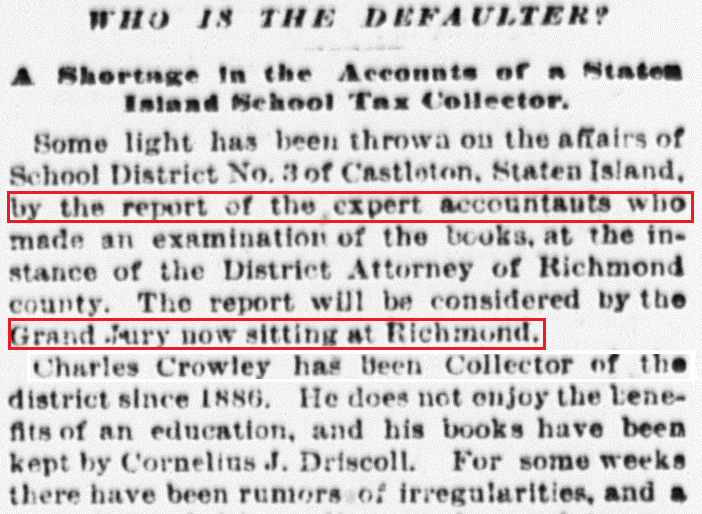
\includegraphics[scale=0.4]{img3}
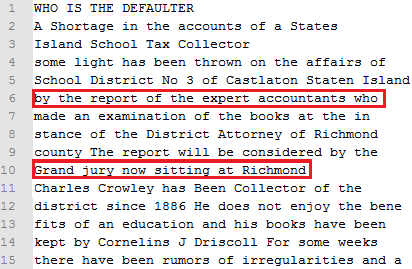
\includegraphics[scale=0.75]{originalimg3}
\caption{Scanned image of a newspape article (left) along with its original text (right)}
\end{figure}
 
\begin{figure}[h]
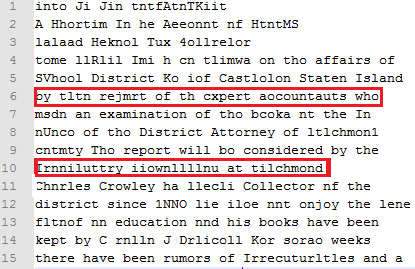
\includegraphics[scale=0.75]{ocr3}
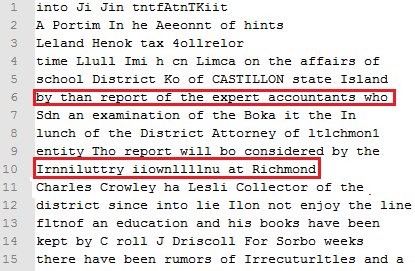
\includegraphics[scale=0.75]{corrected3}
\caption{OCR raw text (left) and Spell corrected text (right) of the article}
\end{figure} 


\textbf{An Example}


Working of the SCE algorithm can be demonstrated with the help of the following example:
Consider 3 versions of a scanned image of a newspaper article,  the original text of the scanned image in Figure 4.2 and the raw OCR text and the corrected text (after spell correction) in Figure 4.3. As highlighted in the figures, for line 6 the line texts are:

 OcrLine= \textit{by tltn rejmrt of th cepert aocountauts who}

CorrectedLine= \textit{by than report of the expert accountants who}

OriginalLine= \textit{by the report of the expert accountants who} 

Here, for each token of CorrectedLine, we find its index and call the MatchWordGrams function accordingly. For the first token 'by' at index i=0 in CorrectedLine, we consider the word window to be "by the report" (index j=0 to 2) in OriginalLine by matching iteratively with each token to see if there is a match and also if there has been a spelling correction by comparing with the corresponding token in OcrLine. Here, no change was made to the spelling of 'by' and it matches with a word in words window, so it is marked as a FN. For the second token 'than' at index i=1, we consider the word window to be "by the report of" (index j=0 to 3) for which there is no match in the window but there has been a spelling correction from 'tltn' to 'than', which implies the correction was wrong and the token is marked as a FP. For the third token 'report' at index i=2, we consider the window as "by the report of the" (index j=0 to 4) in Original Line and find that there is a match in the word window and there has been a spelling correction too from 'rejmrt' to 'report' which makes this token a TP. Similarly, rest of the tokens get marked for each line in the Corrected.txt. 

Another example can be considered from Line 10 in Figure 4.2 and Figure 4.3 where the number of tokens is different in CorrectedLine and OriginalLine. In such a case, direct alignment between tokens is not possible because of which the words window becomes useful. Here, when the last token 'Richmond' of CorrectedLine is considered at index i=3, the corresponding words window becomes "Jury now sitting at Richmond" (index j=1 to 5) for which there is a match in the words windows and corresponding spelling has also been changed from 'tilchmond' to 'Richmond' which makes it a TP. Had the word window not been considered, the corresponding token at index j=3 in OriginalLine would have been chosen as 'sitting' which would have resulted in a FP. 
   


\subsection{Spelling Correction Algorithm Evaluation Results}
\label{spell:eval}

\noindent \textbf{Aims: }The aim of our experiments is to answer the following questions:
\begin{itemize}
\item \textbf{Question 1: }How good is the spell corrector? The metrics for evaluation are accuracy and time to correct the text.
 
\item \textbf{Question 2: }How good is the Person Names Detection Rate? The metric for evaluation is PNDR. 

\end{itemize}

\noindent \textbf{Materials: }
The spelling correction algorithm is used to correct all the 14020 OCR raw text articles in the dataset. The dictionary used for look-up is a concatenation of several public domain books from Project Gutenberg and lists of most frequent words from Wiktionary and the British National Corpus\footnote{http://norvig.com/big.txt}. This is augmented with a large people names list which is obtained  by running Stanford NER-CRF parser on subsets of the ClueWeb12 dataset made available in the TREC 2013 Crowdsourcing Track\footnote{http://boston.lti.cs.cmu.edu/clueweb12/TRECcrowdsourcing2013/}. This enhanced dictionary has been used to give special consideration to correction of person names in the dataset.

\noindent \textbf{Methods: }
In order to answer \textbf{Question 1} we do the following: 

3 versions of each newspaper article are required: OCR raw text, spelling corrector corrected text and the original scanned newspaper article text. Since the dataset is quite large (14020) and it is not possible to get original text of each of these newspaper images, a smaller number of articles are chosen to study the results of spelling correction. 50 scanned newspaper images are taken and an online OCR \footnote{www.onlineocr.net} is run on them followed by some manual correction to get the original articles text. Accuracy can then be calculated for all 3 versions of 50 newspaper articles using the SCE algorithm by marking each word in the OCR text article as a TP, FP, TN or FN. 
%% AAYUSHEE CHECK
%%The dictionary used for the lookup does not contain the large people names list mentioned above.
%%DOUBT--Didnt understand the question

In order to answer \textbf{Question 2} we do the following: 
%% AAYUSHEE CHECK--DONE
\begin{enumerate}
\item Person Name Detection from raw OCR (\textbf{Baseline: }) The NER is run on the raw garbled OCR text.
\item Person Name Detection from spell corrected text (\textbf{PND+Spell Correction: })The NER is run on the spell corrected (using the edit distance algorithm) OCR text without the people names list in the dictionary.
\item Person Name Detection from spell corrected text with enhanced dictionary (\textbf{PND+Spell Correction+Enhanced Dictionary: }) The NER is run on the spell corrected (using the edit distance algorithm) OCR text with the enhanced people names list in the dictionary.

\end{enumerate}

\noindent \textbf{Results: }
The spelling corrector shows an Accuracy of $72.7 \%$  when corrected text is compared to OCR text and original article text. We believe that the results are less accurate due to the presence of a large number of Non-word, New Line, Word Split and Join errors in the OCR data which can not be corrected by the spelling correction algorithm used for this research.

The spelling corrector takes 9 seconds on an average to correct the newspaper OCR articles. It takes a total of 36 hours to run on 14020 articles.

%No need to talk about parallelization here.
%Though the algorithm does not require parallelizing here but it can be parallelized by getting candidate lists for insertion, deletion, substitution and transposition of a word through parallel threads and combining them together for correction of a word.
 
%% Aayushee correct this section using the acronyms defined above--DONE
But the spelling correction is useful in terms of Person Names Detection Rate \textit{(PNDR)}. Following are the statistics obtained for \textit{PNDR}:

\textit{PNDR} for \textbf{Baseline: }: 72.5\% 

\textit{PNDR} for \textbf{PND+Spell Correction: }: 63.3\% 

\textit{PNDR} for \textbf{PND+Spell Correction+Enhanced Dictionary: }: 82.5\% 

These statistics indicate that spelling correction using an extended dictionary for personal names is useful for detecting person names from the garbled newspaper articles and the results are dependent on the type of dictionary being used for spell correction.
 

\textbf{Discussion: }

\begin{description}
\item[$\bullet$]\noindent
A better result can be obtained by correcting the New Line errors in the articles. This can be done by checking for if the word at last index of a text line or the word at first index of the next text line is a word not present in the dictionary and combining the two and checking again in the dictionary for a valid word. The new word, if present in the dictionary can be replaced by the two words from which it is formed thereby removing the New Line error. 
\item[$\bullet$]\noindent Similar approach can be applied for Word Split and Join errors but would require each word of an article not present in the dictionary to be analyzed along with some window of words before and after it to make a correction. 
\item[$\bullet$]\noindent How choice of a dictionary for the edit distance algorithm affects the results still remains to be verified. We believe using a historical dictionary can perform speling correction better and improve the accuracy.
\item[$\bullet$] \noindent Other spelling correction algorithms like context dependent spelling correction can also used to correct the dataset and measure accuracy using our SCE algorithm along with other evaluation parameters to compare among multiple algorithms and decide which one suits the dataset better and gives best accuracy. 
\end{description}



 

\chapter{Development of People Gazetteer}
\label{chapter:people gazetteer}

People Gazetteer as defined in Section~\ref{intro:rc} consists of tuples of person names along with list of documents in which they occur and their corresponding topics. It is developed as an organized structure that can facilitate the process of detection of influential persons from the dataset in an efficient and easy way. This chapter describes the 2-step process of construction of the People Gazetteer by
a) Extraction of person names from the news articles dataset using Named Entity Recognition in  Section~\ref{ner} and
b) Assignment of topics to news articles using LDA topic detection in  Section~\ref{topic detection}.
Output of People gazetteer developed using these steps is presented in Section ~\ref{gaz:result} followed by discussion in Section~\ref{gaz:discussion}

\section{Person Named Entity Recognition (PNER)}
\label{ner}


\subsection{Definition}
NER (Named Entity Recognition) refers to classification of elements in text into pre-defined categories such as the names of persons, organizations, locations, expressions of times, quantities, monetary values, percentages, etc. 
Person Named Entity Recognition (PNER) can be defined as the process of NER that marks up only person names that occur in the text.

PNER is required in this research so as to extract all person name entities occurring in the complete dataset and identify influential person entities among them through development of the People Gazetteer. 
PNER aids in the development of People Gazetteer by first extracting all person names occurring in the dataset followed by reverse linking of a person with the articles in which he/she occurs.

\subsection{Methodology}

The Stanford CRF-NER\footnote{http://nlp.stanford.edu/software/CRF-NER.shtml} is used for PNER in this research. It can perform NER for 3 classes: Person, Organization and Location and is based on linear chain CRF (Conditional Random Field) sequence models. It is trained across several corpora and is fairly robust across multiple domains and even better when compared to some other open source NER systems as illustrated in \cite{rodriquez2012comparison}. According to their results, Stanford NER gave overall the best performance across 2 OCR datasets, and was most effective for PNER when compared with 3 other open source NER systems.


\subsection{PNER Results}
\label{ner:results}
\begin{figure}[h]
  \centering
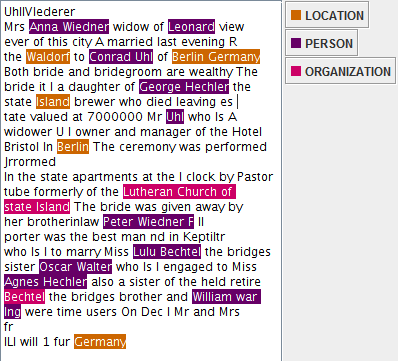
\includegraphics{NER1}
\caption{NER on a sample news article}
\label{figure:sample}
\end{figure} 




NER on a sample news article from the dataset can be seen in Figure~\ref{figure:sample}.
 Stanford NER recognizes a person's full name as separate names by default which is rectified by combining these multi-term entities into single person entities. For example, the person name ``John Smith" is recognized as two separate person entities which we combine to form a single multi-term person entity.
Person names tagged with ``PERSON" category are stored while running NER on the dataset.
Whenever a multi-term person name (number of terms in the person name must be greater than 1) occurs in a document, the person entity's name along with the document name is stored to obtain tuples of person names with their document lists.
The Stanford NER takes 25 minutes to run on the complete news dataset of 14020 articles extracting a total of 38426 person entities. The output obtained can be seen in Table~\ref{table:Table1} which shows the number of person entities with the corresponding number of documents in which they occur.  


\begin{table}[h]
  \begin{center}
\begin{tabular}{|l|l|l|}
    \hline
\textbf{No. of Person Entities} & \textbf{No. of articles} \\ \hline
36615                  & 1               \\ \hline
1122                   & 2               \\	\hline
329                    & 3               \\	\hline
123                    & 4               \\	\hline
87                     & 5               \\	\hline
48                     & 6               \\	\hline
29                     & 7               \\	\hline
19                     & 8               \\	\hline
16                     & 9               \\	\hline
5                      & 10              \\	\hline
4                      & 11              \\	\hline
6                      & 12              \\	\hline
4                      & 14              \\	\hline
3                      & 15              \\	\hline
2                      & 16              \\	\hline
1                      & 17              \\	\hline
1                      & 18              \\	\hline
3                      & 19              \\	\hline
1                      & 20              \\	\hline
1                      & 21              \\	\hline
1                      & 22              \\	\hline
1                      & 23              \\	\hline
1                      & 27              \\	\hline
1                      & 29              \\	\hline
1                      & 31              \\	\hline
1                      & 34              \\	\hline
1                      & 35              \\ 	\hline
\end{tabular}
\end{center}
\caption{Table showing output of PNER on 14020 articles}
\label{table:Table1}
\end{table}



We divide the people entities extracted into following categories so that separate analysis can be done for each category:
\begin{description}
 \item[$\bullet$Marginally Influential]: This category includes all person entities with occurrence in less than 4 news articles. (38066 person entities as calculated from Table~\ref{table:Table1} )
\item[$\bullet$Medium Influential]: This category includes all person entities with occurrence from 4 to 15 news articles. (344 person entities) 
\item[$\bullet$Highly Influential] : This category includes all person entities with occurrence in 16 or more news articles. (16 person entities)
\end{description}
These categories have been created manually simply based on the number of articles of occurrence of a person entity and do not directly lead to the conclusion of a person entity with large number of articles being influential.  


\section{Topic Detection}
\label{topic detection}

 Topic models are algorithms for discovering the main topics that occur across a large and otherwise 
unstructured collection of documents and can organize the collection according to the discovered topics.
Here, a topic refers to a set of words which describe what any document is about.
 A topic model examines the set of documents and discovers based on the statistics of the words in each, what the topics might be and what each document's balance of topics is.
Documents are considered as a mixture of topics and each topic a probability distribution over words.
 Topic detection is the process of identifying topics in a document collection using a topic model. A simple example of topic model illustrated by \cite{blei2012probabilistic} can be seen in Figure~\ref{figure:example}.

Topic detection is essential to this research in order to determine the topics of individual news articles that a person entity occurs in so that the person entity can be linked to the documents in which he/she occurs along with their respective topics.

\begin{figure}[h]
\begin{center}
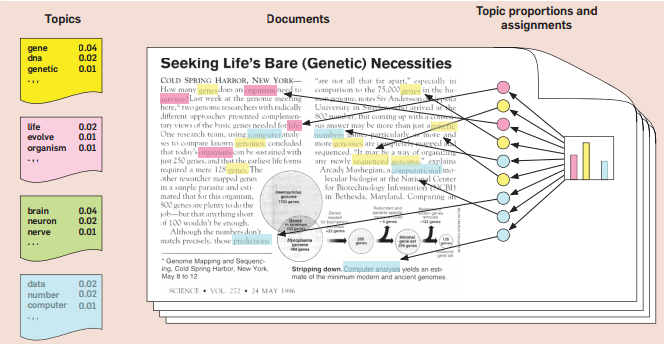
\includegraphics[scale=0.8]{topicmodel}
\caption{Simple topic modelling approach for a single article\cite{blei2012probabilistic}}.
\label{figure:example}
\end{center}
\end{figure} 


\subsection{Topic Detection Model}
\label{topic detection:model}

\subsubsection{Latent Dirichlet Allocation (LDA) Model}

LDA is a generative probabilistic model in which each document is modeled as a finite mixture over an underlying set of topics and each topic, in turn, is modeled as an infinite mixture over an underlying set of topic probabilities\cite{blei2003latent}. In other words, documents exhibit multiple topics and each topic is a distribution over a fixed vocabulary.
The LDA model can be briefly reviewed as follows:


Given an input corpus of $D$ documents with $K$ topics, each topic being a multinomial distribution over a vocabulary of  $W$ words, the documents are modeled by fitting parameters `${\Phi}$' and `${\Theta}$'. `${\Phi}$' is a matrix of size $D \times K$ in which each row is a multinomial distribution of document $d$  indicating the relative importance of words in topics. ${\Theta}$ is the matrix of size $W \times K$ with each column a multinomial distribution of topic $j$ and corresponds to the relative importance of topics in documents.

Given the observed words x = ${x_i}_j$, LDA inference is done by computing the
posterior distribution over the latent topic assignments z = ${z_i}_j$, the mixing proportions ${\Theta_j}$  and the
topics ${\Phi_k}$.  The inferencing is either done using variational bayesian methods or Gibbs sampling which involves integration and sampling of latent variables.
However, the simple LDA approach can take several days to run over a large corpora.


\subsubsection{Distributed LDA Model}
 The simple LDA method takes a long time for topic modeling which is why the distributed version suits large datasets such as ours. The data is partitioned across separate processors and inference is done in a parallel, distributed fashion. 

The Approximate Distributed LDA (AD--LDA) model as proposed by \cite{newman2009distributed} uses distributed computation where total dataset $D$ is distributed equally among multiple $P$ processors. Initialization involves data and parameters distribution to each processor and random assignment of topics so that each processor has its own copy of words $x_p$, topics $z_p$, word topic counts ${{{N_w}_k}_p}$ and topic counts ${{{N_k}_j}_p}$. 
The topic model inferencing then uses simultaneous local Gibbs sampling approach on each processor for a pre-decided number of iterations to reassign topic probabilities $z_p$, word topic ${{N_w}_k}_p$ and topic counts ${{N_k}_j}_p$.
Global update is performed after each pass by using a reduce-scatter operation on word topic count ${{N_w}_k}_p$ to get a single set of counts and obtain final topic assignments.
The model requires user set parameters before inferencing such as number of processors/threads for parallel sampling of data, number of iterations of Gibbs sampling, number of topics and Dirichlet parameters. 

\subsubsection{Topic Models Evaluation}

 Different topic models can be evaluated using the metric of ``Perplexity" which can be defined as how surprised a trained model is when given a held out test data. It has been used in \cite{newman2009distributed} and \cite{blei2003latent} for evaluating the topic detection models under different parameter settings. Perplexity can be calculated using the following formula:

$$Perplexity= \exp(-\dfrac{\text{Log Likelihood of held-out test set}}{\text{Number of tokens in held-out test set}})$$


Here, held-out test set refers to the fact that complete dataset is split into two parts: one for training and the other for testing. The test set is taken as the held-out set for which perplexity is calculated. The document mixture is learned using the training data and log probability of the test data containing unseen documents is computed using the model developed.

Perplexity is a decreasing function of the log likelihood of the unseen documents as can be seen from its formula and lower the perplexity, better is the topic model.

\subsection{Results}
\label{topic detection:result}

The AD-LDA model as described in \cite{newman2009distributed} and implemented in the Mallet\cite{McCallumMALLET} toolkit (known as PLDA model) is used for topic detection over the complete dataset of 14020 news articles. 
Several topic models are first evaluated with different parameter settings in order to pre-decide the number of iterations, processors and topics for the final topic model to be used.


%After training, parameter settings as number of topics varying from 10 to 100, number of iterations from 100 to 500 and number of processors from 1 to 8, the log likelihood of held-out test dataset is calculated along with number of tokens in it to obtain perplexity.

\begin{figure}[h]
\begin{center}
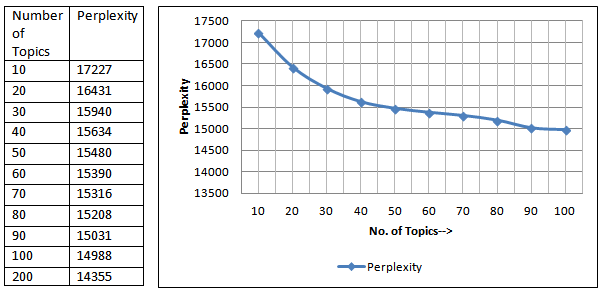
\includegraphics{topicperplex2}
\caption{Test Set Perplexity versus Number of Topics for a random $90-10$ split of the data. The maximum number of words in each topic is $20$, number of iterations $500$ and the number of processors $4$ for this experiment.}
\label{figure:perplex}
\end{center}
\end{figure}

Perplexity is calculated by splitting the data into 90\% for training and rest 10\% for testing. 
Figure~\ref{figure:perplex} shows the variation of the test perplexity versus the number of topics for one random $90-10$ split of the data\footnote{We also vary the number of iterations from 100 to 500 and number of processors from 1 to 8 to study their effect on perplexity. However the number of topics is most influenced by perplexity and hence the other results are not presented here.}. The maximum number of words in each topic is set to $20$, number of iterations $500$ and the number of processors $4$ for this experiment. It exhibits a decreasing perplexity with increase in number of topics. Typically, the number of topics should be chosen as high as possible in order to consider a better model with low perplexity but the model with high number of topics also takes longer to run on a large dataset. The number of topics is set to a value from where further increase in number of topics does not lead to a large decrease in perplexity. We choose the number of topics as $30$ and $100$ and demonstrate their effect on the influential people detection.

From the various topic models and parameter settings, the variability in perplexity with respect to the number of topics has been found to be much greater than the variability due to the number of processors or number of iterations. This is why two values of number of topics are experimented further while number of processors and number of iterations are kept fixed. The number of iterations of Gibbs sampling still need to be above the typical burn-in period of $200$ which is why $500$ is chosen as the parameter value for number of iterations. Number of threads/processors is similarly taken as 4 as least training time is obtained with this parameter value. 

The two models from topic detection are thus used with following parameters:
\begin{enumerate}
 \item \textbf{30 Topics LDA Model} : Number of topics = 30, Number of iterations = 500, Number of threads=4
 \item \textbf{100 Topics LDA Model} : Number of topics = 100, Number of iterations = 500, Number of threads=4
\end{enumerate}
The first model takes 7.5 minutes for training while the second one takes 8.6 minutes.
The set of 30 topics obtained through the first model are illustrated in Table~\ref{table:topicwords} and the other model with 100 topics in Appendix Table~\ref{long}. Some of the topics words can be easily identified to belong to  the following topics: music performance, court events, elections and government and shipping.

Topic modeling gives as output, for each article in the dataset, a set of topics with their probability distribution score for the article. The topic with highest topic probability score is associated with each article in the dataset. 


\begin{table}
\resizebox{15cm}{!} {
 
   \begin{tabular}{|p{1cm}|p{16cm}|}

    \hline
    TOPIC ID & TOPIC WORDS                                                                                                                                           \\ \hline
    1        & total ii won club score night ran furlough alleys tournament time   mile fourth rolled curling scores race national game                              \\ \hline
    2        & la lu ot lo tu au tb ta ha tea day al aa ut ar uu wa tt te                                                                                            \\ \hline
    3        & iii lie tin nail tn lit hut ill ii nn thu tu anti thin inn hit lu lo   nut                                                                            \\ \hline
    4        & line street feet point western easterly northerly feel southerly   distance place distant lo fret hue beginning laid early felt                       \\ \hline
    5        & opera theatre music company week play stage evening night performance   concert mme audience manager season de orchestra house miss                   \\ \hline
    6        & great people life man women good country world american part ot ha   made la years make long place bad                                                \\ \hline
    7        & election mr party republican state district vote democratic county senator   elected city committee mayor political candidate majority york democrats \\ \hline
    8        & time ho work tn men city bo lie anti day thin long thu made part ago   lot york make                                                                  \\ \hline
    9        & st room av sun wife board front lo december rent lot november sunday   ht west ar house private si                                                    \\ \hline
    10       & dr book st story books cloth author cure free work york blood   illustrated remedy goods medical library health price                                 \\ \hline
    11       & church dr father funeral school st college sunday year rev catholic pastor services late service held society holy clock                              \\ \hline
    12       & horse race class horses won racing years prize record year show ring track mile money jockey trotting trotter ran                                     \\ \hline
    13       & cent year week pf market total net stock today central st ft lit sales short cotton ohio lot month                                                    \\ \hline
    14       & white water indian black long found thu big dog time ground wild tree killed birds bird day great lake                                                \\ \hline
    15       & price black silk goods prices ladies worth dress fine white full tea quality style wool made fancy cloth fur                                          \\ \hline
    16       & street mrs mr avenue wife house miss yesterday years home woman night ago husband found died daughter children mother                                 \\ \hline
    17       & war american government army chinese japanese china japan foreign united nov emperor states prince minister military french port navy                 \\ \hline
    18       & feet north minutes avenue boundary seconds degrees west york minute degree point east south feel city angle county laid                               \\ \hline
    19       & man ho men night back wa room left house told bad door found turned place ran lie front morning                                                       \\ \hline
    20       & water feet building boat company car train road fire miles railroad island work line city great river built bridge                                    \\ \hline
    21       & club game team play football half ball left college back yale played harvard line eleven men match yacht field                                        \\ \hline
    22       & ii iii ill lit ll si ti il im vi st iv ft mi li till lull lui oil                                                                                     \\ \hline
    23       & bank money national gold amount notes banks hank business treasury account cent paid bonds note currency company stock estate                         \\ \hline
    24       & mr john william york henry charles james club city ii george dec dr thomas smith jr brooklyn van held                                                 \\ \hline
    25       & piano st rooms car york daily chicago city sunday upright parlor furnished broadway hotel av west train brooklyn monthly                              \\ \hline
    26       & york daily steamship nov directed letter dec fur orleans al steamer walls letters close australia china japan city london                             \\ \hline
    27       & mr court police judge justice case yesterday street district witness jury charge asked attorney trial arrested lawyer told office                     \\ \hline
    28       & mr law present made public year state committee president secretary bill report states con tin united number meeting york                             \\ \hline
    29       & air ran ur fur ui full tt al tl late mr ant liar art lay told met ti tr                                                                               \\ \hline
    30       & company york trust bonds city cent railroad mortgage interest wall bond stock street st central january coupon committee jan                          \\ \hline
    \end{tabular}}
\caption{Table showing Topic ID and words obtained from the 30 Topics LDA model.}
\label{table:topicwords}
\end{table}

\newpage
\section{People Gazetteer Output }
\label{gaz:result}

The list of articles obtained for each person entity after application of PNER and highest scoring topic assigned to each article during Topic Detection are combined to obtain People Gazetteer. In each tuple of the gazetteer, a person entity gets associated with its list of articles where each article is further associated with its corresponding highest scoring topic.

Two people gazetteers are obtained, each corresponding to the two model settings of 30 Topics LDA Model and 100 Topics LDA Model, respectively. A snapshot of the people gazetteer using 30 Topics LDA Model can be seen in Figure~\ref{figure:gazette} where each person entity is followed by a document list consisting of a Document ID and its corresponding Topic ID. A similar people gazetteer is also obtained using 100 Topics LDA Model. Both People Gazetteers are further used in Chapter~\ref{chapter:influential people detection} for detecting and ranking influential person entities from them.
\begin{figure}[!h]
\centering
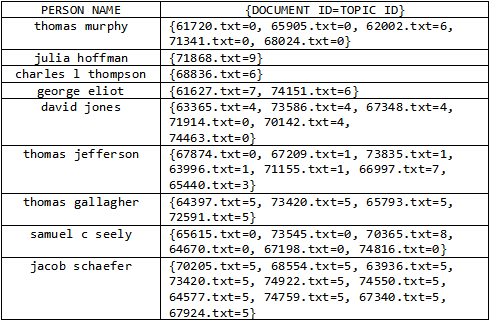
\includegraphics{gazetteer}
\caption{Snapshot of People Gazetteer with Person names, Document list of occurrence and their corresponding Topic ID}
\label{figure:gazette}
\end{figure} 

\section{Discussion}
\label{gaz:discussion}
\begin{enumerate}
\item The Stanford NER, although being one of the best Named Entity Recognizers, is still not able to deal with the dataset of OCR noisy text successfully due to which many of the person entities have been missed and not recognized from the dataset. This can lead to leaving out several potential influential person entities from the process of influential person detection.

\item The OCR text does not contain any punctuation due to which the PNER gives several false positives leading to a large number of garbled person entities in the People Gazetteer. In many cases, either the noisy words get recognized as person entities or they get recognized along with the person entity name making the person name useless for further analysis since it contains extra words in addition to the actual person name. This is one of the main causes of too many unnecessary person entities in the People Gazetteer. It is difficult to identify such people names and filter them out without having a dictionary which contains every possible historical person entity name. Even if all such cases are filtered out, the person entity names which are attached to the noisy words get removed which might remove some important potential influential person entities from further analysis.

\item 
The PNER isn't able to recognize individual entities when multiple person entities are mentioned together without punctuation in the OCR text. They are recognized as one long person entity (false positives get increased) making it impossible to separate out the individual person entities from it. This makes them useless for further analysis and again leads to missing out analysis on potential influential person entities.
For example, in an article with the original line text as: ``They gave money to Ronn, Collector. A. Augustus Healy, Speaker has been appointed..." has the OCR line text as: ``They gave money to Ronn Collector A Augustus Healy Speaker has been appointed.." leading to the recognition of ``Ronn Collector A Augustus Healy Speaker" as one single person entity.

\item
The issues of co-reference resolution of person names (For Example, person entities such as ``William Schmittberger",``Captain Williams" are same but recognized as separate persons) and named entity disambiguation ( Occurrence of different persons with similar name in news articles. For example, the person ``John Smith" detected in two different articles might or might not be the same person) also occur in the People Gazetteer which are not taken care of by PNER and need to be addressed separately. While the issue of co-reference can be still addressed by analyzing each news article, it is extremely hard to disambiguate among persons with similar names that can occur in multiple news articles with different topics.  


\item
The LDA topic detection model is also not geared to be used on OCR dataset directly since it recognizes topics having completely meaningless words. This can be observed from the output of topic detection model in Table ~\ref{table:topicwords} where topics 2,3 and 22 have completely garbled words.

\end{enumerate} 

\chapter{Influential People Detection}\label{chapter:influential people detection}



\section{Related Work}
\label{influential:rw}

influential ppl done in social media 
learning through cascades
connecting the dots paper




gossip based algo
l
http://www.cs.cornell.edu/home/kleinber/

http://cs.stanford.edu/people/jure/




dont necessarily use cascades
will that work in this setting?
do cascades also work in my environment

\section{Measuring Influence}
\label{influential:measure}
2 subheading: measure influence of individual article
measure influence of individual entity

define parameters
procedure for finding Influence score for each article

\section{Ranking}
\label{influential:ranking}

\section{Results}

statistics table regarding each category of person entities
ranking
how document parameters affect chains
how lda affects chains
take each person from the three categories
visualization using google visualization toolkit?
\subsection{Case Studies}

influential person detection based on topics also
change of topic detection parameters
       
\section{Conclusion}
discussion on results 

The set of topics derived from a corpus can be used to answer questions about the similarity of words and 
documents: two words are similar to the extent that they appear in the same topics, and two documents are similar to 
the extent that the same topics appear in those documents. 
                                                           

%\newpage
%\bibliographystyle{these}
\bibliographystyle{acm}
%\bibliographystyle{elsart-harv}
%\newpage
%\section{References}
%\bibliography{Library}

\bibliography{aayushee}
\chapter*{Appendix}\label{chapter:appendix} 

\end{document}
